\documentclass[twocolumn,10pt]{article}
\usepackage[utf8]{inputenc}

\usepackage{lipsum}
\usepackage[top=1in, bottom=1in, left=1in, right=1in]{geometry}
\usepackage[numbers]{natbib}
% \usepackage[,style=ieee,natbib=true]{biblatex} %added

\usepackage{amsmath}
\usepackage[pdftex]{graphicx}
% declare the path(s) where your graphic files are
\graphicspath{{./img/}}

\title{State-based Markov Feature Learning for Gas Turbine Anomalies}
\author{Thurston Sexton \& Connor Armstrong}
\date{December 15, 2017}
\DeclareMathOperator*{\argmin}{argmin}

\begin{document}
\maketitle

\section{Introduction}

Gas turbines are the beating hearts of modern industry, by converting a variety of fuels to electrical current they are capable of producing up to 225 MW of power. These incredibly complicated systems are vital to the function of factories and homes, meaning any unscheduled downtime is unacceptable. Traditionally, the most popular way to identify turbine anomalies is monitoring exhaust gas temperatures (EGTs) exiting combustion chambers. Traditional approaches are reliant upon rigid handcrafted features derived from prior engineering knowledge. Knowledge-based features are hindered by poor predictive performance, and crafting "good" features is an extremely time-consuming manual process. Improving the versatility and accuracy of anomaly detection requires a feature learning solution capable of autonomously creating efficient features from raw data. 

\subsection{Existing literature}
%List any major feature learning and/or prediction approaches out there that might specifically apply to sensor/turbine anomaly prediction. We want to end up talking about the methodology in \citep{gas_turbine} and how we're extending it. e.g: 

Previous studies on anomaly detection in gas turbines have investigated the effectiveness of supervised and unsupervised prediction methods on fixed data sets; however feature learning is rarely discussed \cite{yan2015}. 

A prior gas turbine study by Yan and Yu \cite{yan2015} indicated semi-supervised feature learning may be used to improve classification. Learned features supplied training inputs for an extreme learning model (ELM). Feature learning was facilitated using a stacked denoising autoencoder (SDAE); a deep learning structure which has a denoising autoencoder (DAE) for shallow learning blocks. DAEs are a variant of the traditional auto-encoder. AEs consist of an encoder and decoder component. An encoder function maps inputs to hidden representations, whereas a decoder function maps those hidden representations to a reconstruction \cite{yan2015}. DAEs are trained to fill in missing data, which relies upon the predetermined AE activation function to classify features. The ELM is trained by finding connections from hidden neurons to output neurons using a single design parameter. However, interpreting these learned features tends to be incredibly difficult, and it is desirable for engineers to understand \textit{why} a particular anomaly prediction was made.

As discussed in Li et al. \cite{gas_turbine}, Hidden Markov Models (HMMs) can be used for turbine anomaly detection in either semi-supervised or supervised settings, by encoding a wide range of system behavior into state transition probabilities. Knowing that turbines are going to have particular ``states" like ``on" or ``off" or ``warming", along with how we expect the states to transition from one to another, lets us directly encode that information into a HMM's network. Additionally, HMM's naturally calculate the probability of observed time-series, once trained. However, using HMM models this way generally requires specific domain knowledge about ``useful" parameters, like \textit{how many states exist for this system?}, or perhaps more importantly, \textit{what time-scale do anomalies occur in for this system?}. 

\subsection{Project Overview}
In this project, we propose a method to extend the work of Li et al. \cite{gas_turbine}, by automatically determining optimal settings for a HMM that is able to 1) model the overall system behavior in a human-interpretable way, and 2) predict the occurrence of anomalies in both a supervised and semi-supervised way. 
This will be achieved through:
\begin{enumerate}
    \item Automatic extraction of state emission probabilities by clustering observed temperature sensor records
    \item Determining optimally-predictive sequence-time windows and number of system states through Bayesian Optimization, and
    \item transformation of the original features into a ``probability feature-space", which can be used for supervised or semi-supervised anomaly detection. 
\end{enumerate}

This methodology will be demonstrated through application to detecting anomalies in a real data-set.

\section{Sensors as State Sequences}
To learn useful features for time-series data, it is necessary to make some assumptions about how the time-series is structured. For example, using wavelet transforms \cite{yan2015} implies a frequency-cutoff assumption to restrict the feature domain size. The goal of \textit{feature learning} is to minimize the number of assumptions required to get ``useful" features for prediction -- i.e. to prevent \textit{feature engineering}. We propose that, by only assuming that there exist separate ``operational states" of the system, that it is possible to learn features derived from sequences of these states. This is accomplished through the use of Hidden Markov models, to map the observed sensor values to one of the ``hidden" states. These mappings can then be used to determine the relative probability of some given sequence of states, based on what has been observed before.

One way to view this HMM mapping of continuous sensor measurements to sequences of states is as a \textbf{Mixture Model}, where each component of the mixture represents one of the ``states" the system can be in, with each component's distribution representing the ``emission probability" of sensor values while in that state. These components are then related through a transition probability matrix, which allows the system to shift into different components of the mixture model over time. 

\subsection{Mixture Model}\label{sec:gmm}
Mixture models are generalized distribution functions created by combining two or more individual, weighted probability distributions. When these are assumed to be Normal distributions, this is called a Gaussian Mixture Model (GMM). For $K$ components, each with one of the weights in a (unit-norm) weight vector $\phi$, the GMM is defined as:
\begin{equation}\label{gmm}
    p(x) = \sum_{i=1}^{K} \phi_i\mathcal{N}(x|\mu_i, \sigma_i)
\end{equation}

These are useful when, given some $K$, one is able to ``fit" a GMM's parameters $\theta=(\phi, \mu, \sigma)$ to some empirical data distribution, giving an un-supervised probabilistic ``clustering" of our data. There are several ways to calculate these parameters. Though in practice, expectation maximization works well given some initialization through, say, K-means clustering.~\citep{GMMfit} 
\footnote{K-Means Clustering is a useful tool for classifying unlabeled data. Classification is based upon a user-selected number of clusters ``K" data will be classified into. The number of clusters ``K" is associated with the number of visible \textit{states}. Simple classification, first discussed by Lloyd, is based upon constant optimization of cluster centroids \cite{pcm} . Unfortunately, this makes K-Means susceptible to noise. For the purposes of this investigation, K-Means Clustering is implemented when using both Gaussian Mixture Models and HMM's}

Once trained, it is possible to to calculate the probabilities of component membership for some in-coming data point, $P(\theta_i|x)$,  using Bayes-rule. However, these are state-independent, meaning that any probability of an observation being in a state is completely independent of the previous observation's state. This is undesirable for time-series modeling, leading to the generalization into HMMs.

% The generated Gaussian components of the function are referred to as ``modes". Mode density must be selected carefully, as too few will result in under-fitting, whereas too many will over-fit the sum. To preclude this, components can be be dynamically added or removed depending upon their relevance to updating data \cite{GMM}. Creation of discrete modes is shown to be an effective means of separating data by Zivkovic through image processing applications \cite{GMM}.


\subsection{Training an HMM}

Given the previously described structure of mixture models, we would like to implement a model that observes the Markov property, namely, that the probability of some state is solely dependent upon the current state's transition probabilities (Figure \ref{fig:HMM exmaple}). Therefore, it remains to determine the transition probability matrix for moving between our components, which is done by observing known sequences of states and updating the mixture component parameters with the associated transition matrix through expectation maximization in both the forward and backward time-direction. This is known as the Baum-Welch algorithm, or alternatively ``forward-backward training", and is implemented in most HMM packages.~\citep{baum-welch}

\begin{figure}
    \centering
    \includegraphics[width=\linewidth]{img/"HMM transition".png}
    \caption{Example of a Hidden Markov Model \\
    \centering X -  hidden states \\
        y - observations \\
        a - transition probability \\
        b - observation probability\\
        \tiny{Image by Tduning, distributed under a CC-BY-3.0 license.}}
    \label{fig:HMM exmaple}
\end{figure}

% .\citep{pomegranate}

% \subsection{HMM State Prediction}
% here we will plot the example breakdown of some sensor signal into states (maybe a sensor time-series colored by the predicted HMM state?)

\subsection{Learned Probability Features}
Once the transition and emission probabilities are trained for each state of the HMM, one might want to know the probability (or more commonly, the log-probability) of some new observed sequence. One way might be to calculate the log-probability of the ``most likely" state path the observed sequence might take. This is the \textit{Viterbi} probability. However, the get the overall probability we must additionally sum over all \textit{possible} paths, not simply the most likely (Viterbi) path. 

It is important to note that this probability value represents a sequences probability, and not a single point in time. At this point, we must interpret what it means for a point in time to be ``anomalous". Because a system state (and by extension, our observations of it through sensors) must inherently depend on the some previous system state (observable through previous sensor measurements), we posit that on might define a point as anomalous if the prior sequence of observations is relatively less likely. This must be calculated within some time-window, which would define the time ``length-scale" of the system whereby anomalies happen. 

If a time-scale window is given, one can then define the Markov probability feature $f_P$ of a set of time-series data in the set of possible times $t\in T$, using a trained HMM $M$ with $K$ states, as: 
\begin{equation}
    f_P(t|K, W) = \log P_M(\{s\in T | t-W \leq s\leq t \}, K)
\end{equation} 
where $P_M$ the log-probability of a the given set of observations in window  $W$, as detailed above. Intuitively, this means we assign a low probability to some observation in time \textit{if the preceding sequence of observations were unlikely}. In this way, it is possible to create a probability feature through a unique HMM for every sensor in the original measurements' feature-space. 


\subsection{Learning}

To avoid ``engineering" the parameters $(K, W)$ of the Markov probability feature function, we pose the feature learning problem as an optimization problem: the minimization of loss over the space of hyper-parameter values $(K, W)$. In this way, we do not need to provide either as a priori information, but only a range of feasible or desired values for them to take (i.e. the bounds). To do this, we first use an un-supervised anomaly detection scheme to label probabilities as anomalous or typical. Then, we define a loss function based on the $F_{\beta}$-score. 

\subsubsection{Anomaly Detection}
In Li et al. \cite{gas_turbine}, simple threshold values were used to determine a proper probability, below which some set of observations would be considered anomalous. However, this requires a great deal of intervention on the part of a modeler, since each sensor HMM may capture the probability of states differently. Instead, we exploit the fact that our probability features are, by design, largely stationary 
\footnote{That is, unlike the original sensor which might exhibit sharp increases in value (e.g. sharp temperature increase) or change over time (extended regions of non-zero net-slope), probabilities will inherently remain in the region $[0,1]$ }
and that the density of low-probability sequences, as determined by a HMM trained on this data, should be much lower than the relative density of medium and high-probability sequences. With this in mind, we use a Mahalanobis Distance (MD) anomaly detection scheme (also called an Elliptic Envelope) to determine which observations are, in fact, anomalously low-probability. The MD is a higher-dimensional, weighted generalization of euclidian distance, where it is assumed that the data is normally distributed. defined in terms of a Gaussian mean (location) $\mu$ and covariance matrix. The covariance matrix defines a MD for every sample point from the mean location.

\subsubsection{Hyper-Parameter Optimization}
There are several ways one might define ``loss" to minimize over, but here we will take two observations into account: 1) it is generally more important to catch an anomalous system state than it is to predict typical states as anomalous, and 2) this is only true so long as the topology of the prediction is preserved (e.g. predicting two anomalies in a region of order $|W|$ when only one exists is fine, but predict all points as anomalous is useless. 

This intuition is essentially balance of Recall and Precision, i.e. the ability of an information retrieval scheme to \textit{not miss true labels} and to \textit{not mis-label}, balanced in some way. the $F_{\beta}$-score is the harmonic mean of Recall and Precision, weighted to prefer Recall $\beta$-times more than precision. Following the above, we adopt $\beta=2$ as a heuristic to capture the previous assumptions. 

With such a metric, we can score the quality of the anomaly detection described previously as compares to a known set of anomaly observations, and define our feature-learning problem as 
\begin{equation}\label{eq:obj}
    f^*_P(t) = \argmin_{K, W} F_2({\rm MD}(f_P(t|K, W)), y(t))
\end{equation}
where ${\rm MD}$ is the mahalanobis-distance-based anomaly detection scheme discussed above, and $y(t)$ is the ``true" observed state of the system at time $t$ (anomalous or not). 


\section{Results}

%The method above was applied to turbine temperature sensor data, collected over X months at a sample rate of Y. In all, Z anomalies were known to occur during this period. 

The method above was applied to turbine temperature sensor data from 27 separate combustion chambers within a single gas turbine (listed as individual columns labeled ``T$\_$1" through ``T$\_$27”). Temperature readings were recorded once a minute during three collection intervals. The first collection interval (6302) spanned from April 1st to August 20th 2010, the second (7600) from May 1st to August 20th 2009, and the final (7664) from February 1st to April 30th 2010. There is a vast abundance of data considering the mentioned sampling interval (204475 , 161276 , & 128157 samples respectively).

According to the ground truths of the data, there are only
27 identified fault events across all three collection intervals. Said faults only occur at single time
samples, meaning the identified fault events are point anomalies in the data. However, this
implies that 99.99 \% of the provided data could be considered “healthy”, a major class imbalance

\subsection{Method}
For this case study, original signals were up-sampled to 4-hour interval means, to reduce the computational complexity of the task these signals, along with the deviations from the overall mean signal at each point are shown in Fig.~\ref{fig:signals}.
\begin{figure*}
    \centering
    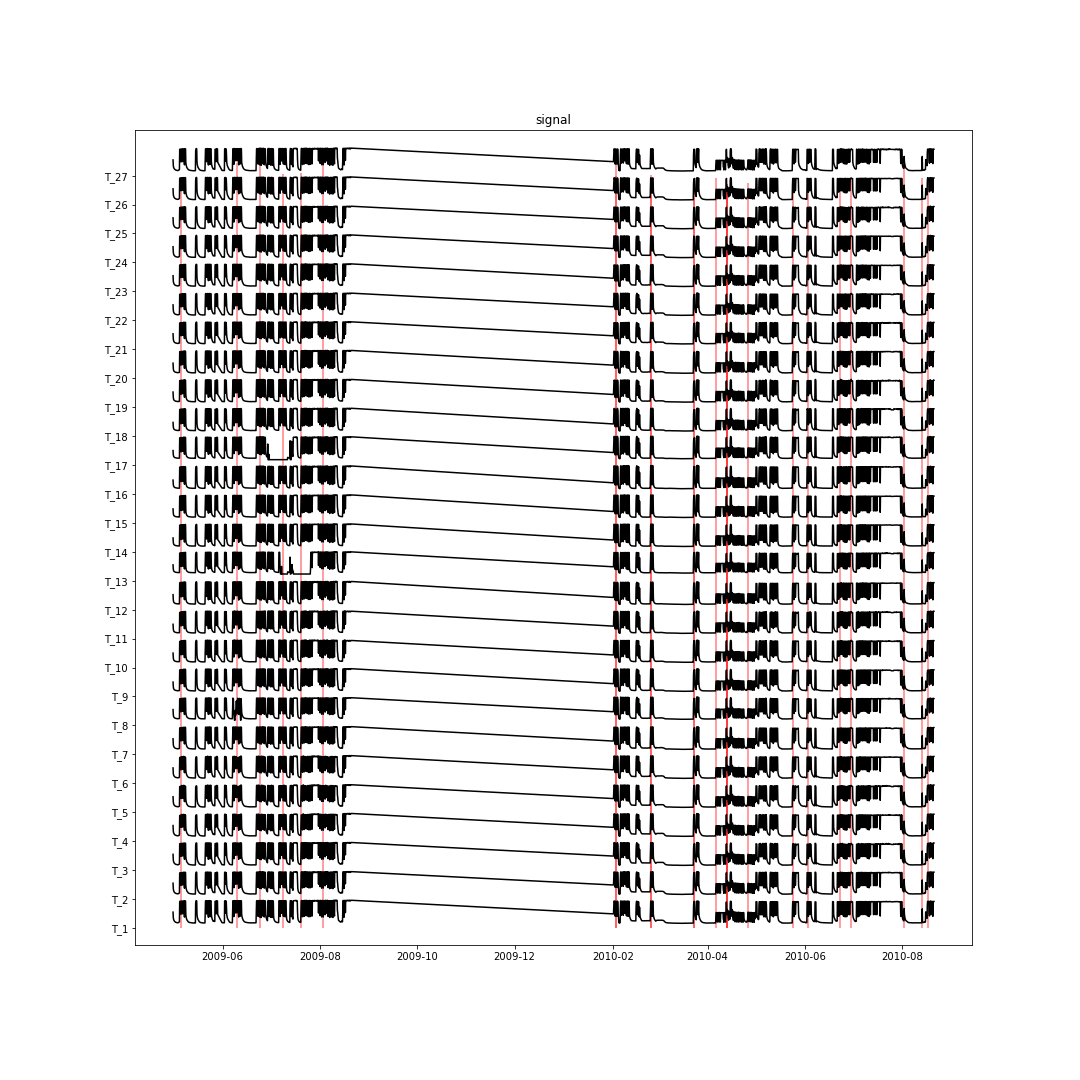
\includegraphics[width=\linewidth]{img/signal_plot.png}
    \caption{Left, demonstration of data used for this anomaly detection case study. Sensor data has been up-sampled to a 4-hour ``compression window" for computation considerations. Right, since all sensors appear very similar, deviations from the mean-signal are shown for each sensor. Known anomaly times are shown in red. }
    \label{fig:signals}
\end{figure*}

\subsubsection{HMM Instantiation}
To fit a HMM model via Baum-Welch, a given $(K,W)$ parameter pair was used to split the up-sampled data into (rolling) sequences of duration $W$, and passed into a $K$-state HMM model fitter. The open-source python package Pomegranate~\cite{pomegranate} was used to create such a $(K,W)$-HMM model, which will assign hidden-state labels to each sequence observation, assigning the sequence to a reference time (the last time-stamp in the sequence). Such a state-labeling is shown in Fig.~\ref{fig:states}. 

\begin{figure*}
    \centering
    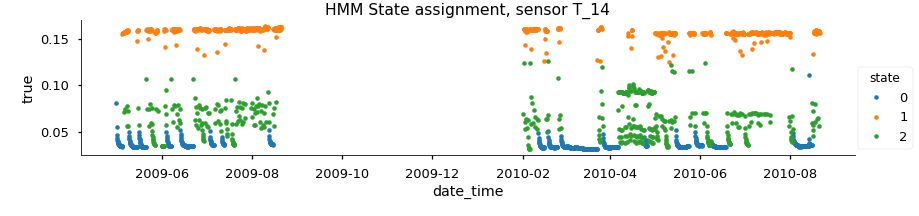
\includegraphics[width=\linewidth]{img/true_hmm_state.png}
    \caption{Predicted state labels for $(K=3, W=5{\rm h}$ ( the optimal hyper-parameters as determined by BO), for an example sensor (Sensor $T_{14}$ was determined to have the highest $F_2$-score for these settings).}\label{fig:states}
\end{figure*}
To ensure that the HMM model's learned emission and transition probabilities would suggest low sequence probability when \textit{containing} an anomaly, sequences of size $W$ known, a priori, to contain anomalous behavior were omitted from the training sequence set. This may not be necessary, since anomalous system states should be, de facto, rare. Therefore the probability of sequences containing them should be consequentially low. This would be a true unsupervised method, whereas, insofar as one must know which states are anomalous in order to omit them, the method described here is somewhat of a \textit{semi-supervised} approach. 

\subsubsection{Optimization}
Because training multiple HMM's\footnote{One for each sensor, aggregated, and repeated for each evaluation of the objective function in Eq.~\ref{eq:obj}}  is computationally costly --- increasingly so for larger numbers of states --- we use Bayesian Optimization (BO) to minimize the loss. BO uses Gaussian Process Regression (GPR) to approximate a posterior distribution of the true objective function we are trying to optimize (both a mean-function and a standard deviation on it --- our expectation and our uncertainty, respectively). The goal is to provide global convergence in as few iterations of the true objective function as possible, usually by predicting where might provide the greatest improvement of the surrogate fit. This is done by optimizing an acquisition function, derived from the $\mu, \sigma$ functions, and might take the form of maximizing \textit{Expected Information Gain} (EI), \textit{Lower Confidence Bound} (LCB), etc. Space does not permit an in-depth analysis of BO here, but it has shown great ability to quickly converge on good optima for a relatively few number of objective function evaluations --- in fact, it is often known as Efficient Global Optimization in engineering design.~\citep{efficient-global-opt}

This project used a Gaussian Process BO, predicting each successive sample by optimizing the LCB via L-BFGS-B.~\cite{zhu1997algorithm} The algorithm was initialized with 5 radom objective samples, via latin-hypercube sampling.~\cite{eglajs1977new} Minimization of the negative of Eq.~\ref{eq:obj} was performed using the GPyOpt package\cite{gpyopt2016}. Convergence behavior and ultimate shape of the $\mu$, $\sigma$, and aquisition functions is shown in Fig.~\ref{fig:BO}


\begin{figure*}
    \centering
    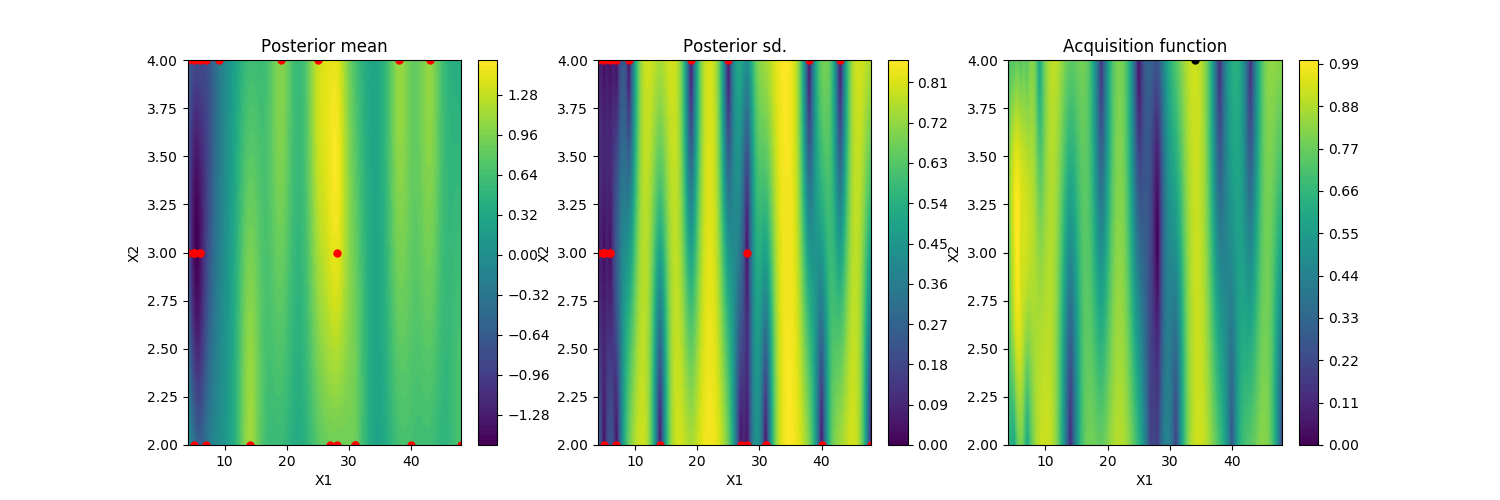
\includegraphics[width=\linewidth]{img/acq.png}
    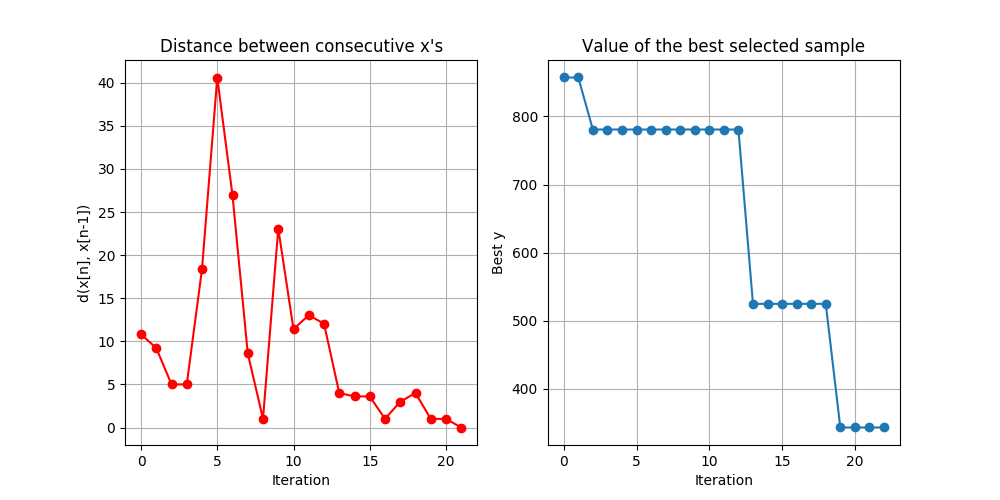
\includegraphics[width=.7\linewidth]{conv}
    \caption{BO performance for minimizing the negative of Eq.~\ref{eq:obj} over $K$ (X2) and $W$ (X1). Upper right shows the posterior mean-function, which is our surrogate for the model score at a given combination of $(K,W)$. Note the nearly oscillatory behavior along the $W$-axis, indicating that length-scales near 24, 32, and 48-hours seem to be more predictive than others --- this makes sense given the natural schedules in the workplace. 3-states appears to be (barely) best at capturing system behavior, of the three options available (restricted due to computational complexity and time). Bottom plots indication convergence behavior of BO, in minimizing $-F_2$. }
    \label{fig:BO}
\end{figure*}

For time and computational effectiveness, the range of search was limited to 2,3, or 4 states, in combination with between 4 and 48 hour time-window/length-scales. Though restrictive, it is possible in principle to search over a much larger area given additional time, and parallelization of objective evaluation. Still, converging after 24 iterations is exceedingly better than the full 126 evaluations required for a full search. The optimal settings found were $K=3$ states, and $W=5$ hour window, respectively.

\begin{figure*}
    \centering
    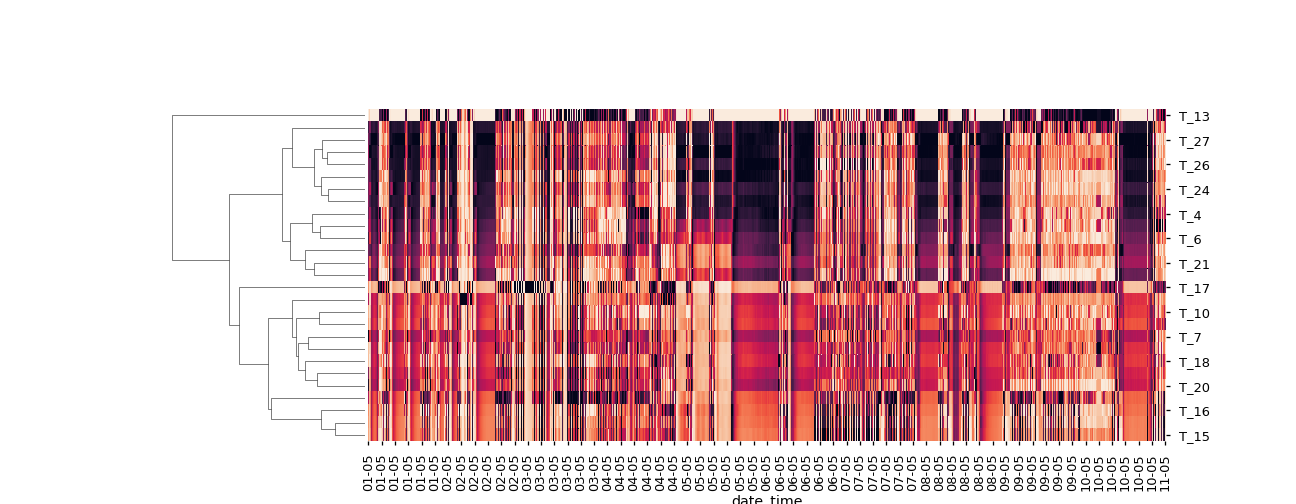
\includegraphics[width=\linewidth]{cluster_prob.png}
    \caption{$f^*_P$ for each sensor's HMM model: darker indicates lower probability. Hierarchically clustered to demonstrate the core classes of sensor types, natrurally derived by the sequence probabilities determined by HMM. Note T13 and T17, both of which appear to be largely in disagreement with the probability assessments of the rest of the sensors.  }
    \label{fig:my_label}
\end{figure*}


\subsection{Semi-supervised}
As mentioned previously, because our probability features are stationary signals, we may use a Mahalanobis-distance anomaly detection scheme directly on the entire time-range, determining which times are unlikely and, therefore, anomalous. First, using the fact that our optimization has derived a natural time length-scale of $W=$ 5 hours, we flag all times within any 5 hour period as anomalous if an anomaly was contained in that window. The contamination factor for anomaly detection was then set to the ratio of total anomalous times to total (up-sampled) measurements, or about $1.1\%$ The times flaged as anomalous with this semi-supervised method are shown in Fig.~\ref{fig:unsupervised}

Additionally, it is possible to train a higher-dimensional MD-anomaly detector, by training on the 27-dimensional input of \textit{all probability features}. This sacrifices specificity, where a given sensor may ``know" something about a particular anomalous region in our system, while providing generality about interaction between all sensors. This is also in Fig.`\ref{fig:unsupervised}, labeled as ``combined".
% Things lag...our predictions are consistently behind/just after the actual occurrence of anomaly, Fig.~\ref{fig:unsupervised}. This does mean we are learning some deeper, useful abstraction of the system behavior, but we need to re-parameterize or redefine our objective function so that things are predicted at the right time...
\begin{figure*}
    \centering
    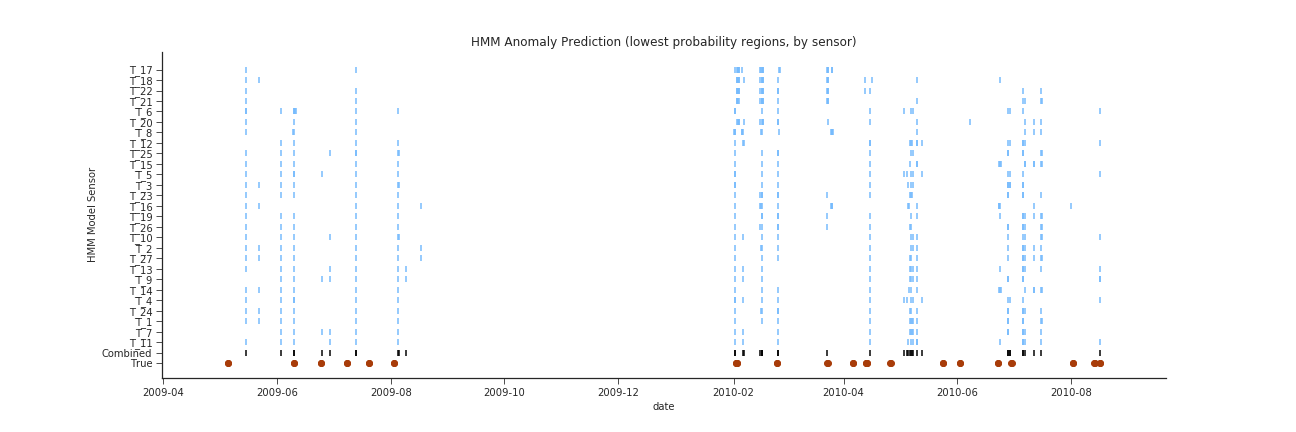
\includegraphics[width=\linewidth]{unsupervised.png}
    \caption{Markers MD-predicted anomalies occurring at this time, using a contamination factor equal to the empirical contamination factor of the true labels. Sensor models are ordered from bottom (best score) to top (worst score). The ``combined" predictions were done in a higher(27)-dimensional feature-space containing the $f_P$ transformations for all sensors.  }
    \label{fig:unsupervised}
\end{figure*}

\subsection{Supervised}
Finally, it is also possible to train a supervised model on the probability features, which might provide a sort of benchmark for comparison to the prediction ability of the original ``raw" feature-space (the original sensor signals). A decision tree was trained over 5 train-test folds\footnote{These splits were performed in a way that preserved chronology of the time-series.} with a maximum depth of 27 branchings. The $F_2$-score results for 100 trials is shown in Fig.~\ref{fig:tree_fscores}
% Use the probability features as input into a decision tree or SVM, instead of the original sensor data. We will do cross-validation, but making sure the "training" sets are always time-points \textit{before} the test sets. See how well that does? Fig.~\ref{fig:supervised} 

\begin{figure}
    \centering
    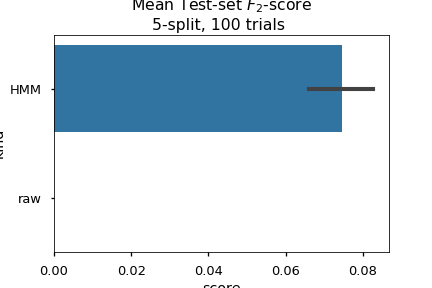
\includegraphics[width=\linewidth]{img/tree_fscores.png}
    \caption{Mean $F_2$ scores of a Decision-tree model with maximum depth of 27 (allowing at least one split per sensor, if needed), over 100 repetitions of a 5-fold time-series-split used for cross-validation. Raw signals were unable to achieve a non-zero $F_2$-score. }
    \label{fig:tree_fscores}
\end{figure}

\begin{figure}
    \centering
    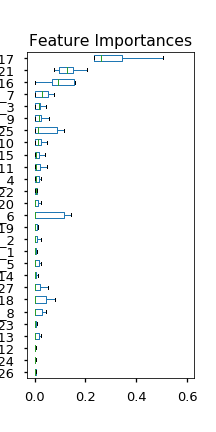
\includegraphics[width=.7\linewidth]{img/tree_imp.png}
    \caption{Feature-importances of best-performing Decision tree w.r.t. $F_2$-score. }
    \label{fig:tree_importances. }
\end{figure}

\section{Conclusions}


Based upon the accuracy of the MD anomaly prediction scheme for each sensor's HMM it is clear that the learned features are often appropriate for anomaly classification. Analysis of the semi-supervised method accuracy in Fig. \ref{fig:unsupervised} identifies the most important features at the bottom of the y axis. The most important feature for the semi-supervised method being $T\_14$. The higher-dimensional ``combined" predictions performed comparatively worse than the individual ones. It is also worth noting the improvement in the first ``phase" of system activity in Figure \ref{fig:unsupervised} at the cost of accurate predictions in the second.

The supervised decision tree benchmark in Figure \ref{fig:tree_fscores} (HMM versus raw signals) confirms that the HMM inputs had a more accurate prediction ability than the raw data, which was completely indecipherable to the DT. Curiously, the most important feature identified by the DT in Figure \ref{fig:tree_importances. }, $T\_17$, differed from the most important feature identified by the semi-supervised model ($T\_14$). In fact Figure \ref{fig:tree_importances. } indicates the difference in importance between $T\_14$ and $T\_17$ is massive. 

Overall, we were pleased to see an improvement in model performance from the interim report. However, it was observed that model predictions lagged behind true anomalies. To prevent this, further investigation and re-definition of optimal time windows are required.


% It does OK...more do well, but more do poorly too. This indicates there is some minimum amount of time the model needs before the probabilities are useful. This model either does great or terrible, while before it was a whole lot of mediocre. 

% \section{DEFINITION STUFF}
% I just put things you had into a section to be sorted later. 
% \subsection{Terms I don't know if we need anymore}

% \subsubsection{Support Vector Machine}\cite{SVM}
% The Support Vector Machine (SVM) is a commonly used binary-classification tool. A pure, hard-margin SVM is ideal for data that is linearly separable. However we didn't really use this, did we?

% \subsubsection{Singular Value Decomposition}
% Singular Value Decomposition (SVD) is a method of data dimensional reduction. It's useful, but I don't know how relevant it's going to be if we use the ``swinging door" compression thing.

% \subsubsection{Principle Component Analysis}
% Did we use this for anything other than justification? Is it worth talking about anymore?

% \subsection{K means clustering}\label{sec:kmeans}
% K-Means Clustering is a useful tool for classifying unlabeled data based. Classification is based upon a user-selected number of clusters ``K" data will be classified into. The number of clusters ``K" is associated with the number of visible \textbf{symbols/states}\footnote{from here on ``symbols" will be used}. Simple classification, first discussed by Lloyd, is based upon constant optimization of cluster centroids \cite{pcm} . Unfortunately, this makes K-Means susceptible to noise. For the purposes of this investigation, K-Means Clustering is implemented when using both Gaussian Mixture Models (Section \ref{sec:gmm}) as well as Hidden Markov Models (Section ~\ref{sec:hmm}).

% \subsection{Gaussian Mixture Model}\label{sec:gmm}
% When working with functions such as Fig. (normalized temperature density), it can be useful to interpret them as the sum of Multiple Gaussian distributions. The generated Gaussian components of the function are referred to as ``modes". Mode density must be selected carefully, as too few will result in under-fitting, whereas too many will over-fit the sum. To preclude this, components can be be dynamically added or removed depending upon their relevance to updating data \cite{GMM}.

% The number of modes in a function can be considered the number of visible symbols, and is used as the ``K" value as discussed in Section \ref{sec:kmeans}. Creation of discrete modes is shown to be an effective means of separating data by Zivkovic through image processing applications \cite{GMM}.
% Computing the appropriate number of visible symbols will be discussed in Section.

% \subsection{Hidden Markov Model}\label{sec:hmm}



\bibliographystyle{ieeetr}
\bibliography{biblio}
\end{document}
